\documentclass{jsarticle}
\usepackage[dvipdfmx]{graphicx}
\usepackage{bm}
\usepackage{amsmath}
\usepackage{amssymb}
\usepackage{amsfonts}
\usepackage{comment}
\usepackage{listings}
\usepackage{cases}
\usepackage{siunitx}
\usepackage[hyphens]{url}
\lstset{
    basicstyle={\ttfamily},
    identifierstyle={\small},
    commentstyle={\smallitshape},
    keywordstyle={\small\bfseries},
    ndkeywordstyle={\small},
    stringstyle={\small\ttfamily},
    frame={tb},
    breaklines=true,
    columns=[l]{fullflexible},
    numbers=left,
    xrightmargin=0zw,
    xleftmargin=3zw,
    numberstyle={\scriptsize},
    stepnumber=1,
    numbersep=1zw,
    lineskip=-0.5ex,
    keepspaces=true,
    language=c
}
\renewcommand{\lstlistingname}{リスト}
\makeatletter
\newcommand{\figcaption}[1]{\def\@captype{figure}\caption{#1}}
\newcommand{\tblcaption}[1]{\def\@captype{table}\caption{#1}}
\makeatother

\title{運動を3D化する技術}
\date{}

\begin{document}
    \maketitle
    \section{MAC3Dシステム}
        MAC3Dシステムは人体にマーカを貼り付け、
        専用のカメラを複数使い、運動の様子をすることでその動きを3D化する。

        \begin{figure}[h]
            \begin{minipage}{0.5\hsize}
                \centering
                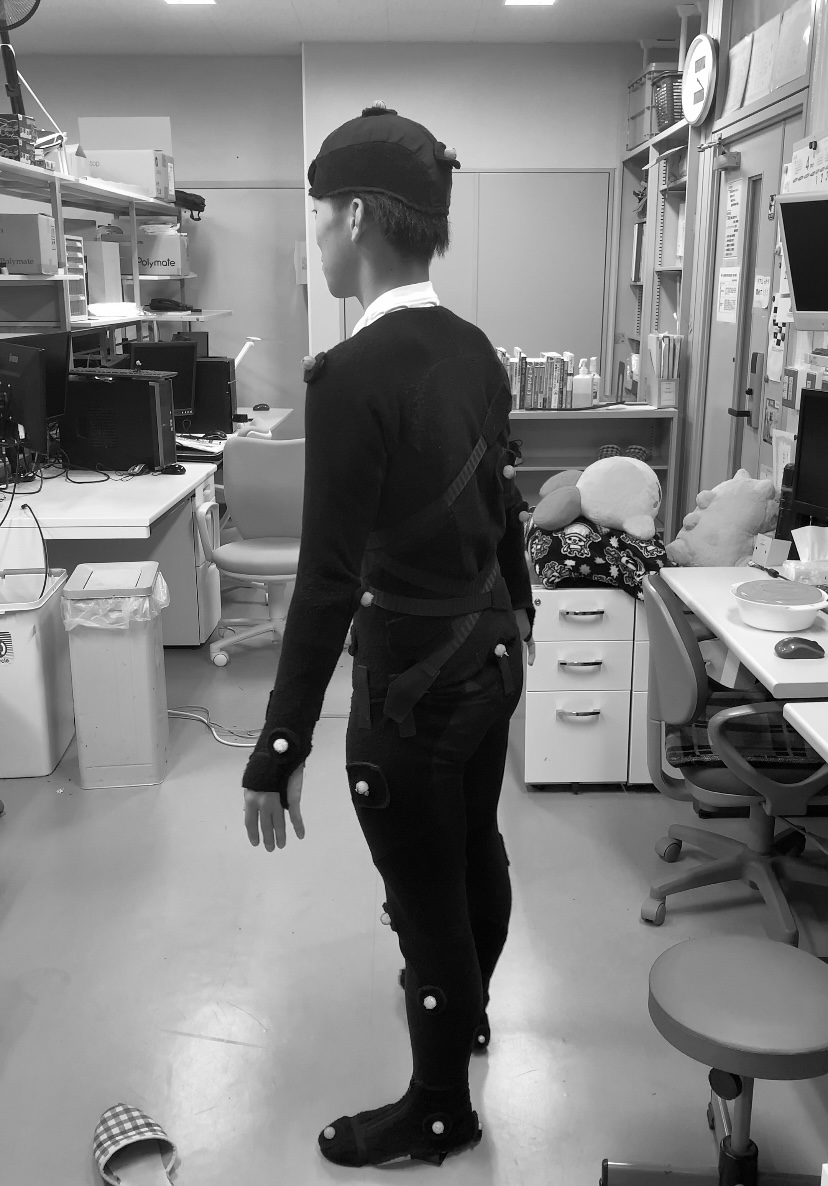
\includegraphics[width=0.9\hsize]{img/marker.jpg}
                \caption{被計測者の様子}
            \end{minipage}
            \begin{minipage}{0.5\hsize}
                \centering
                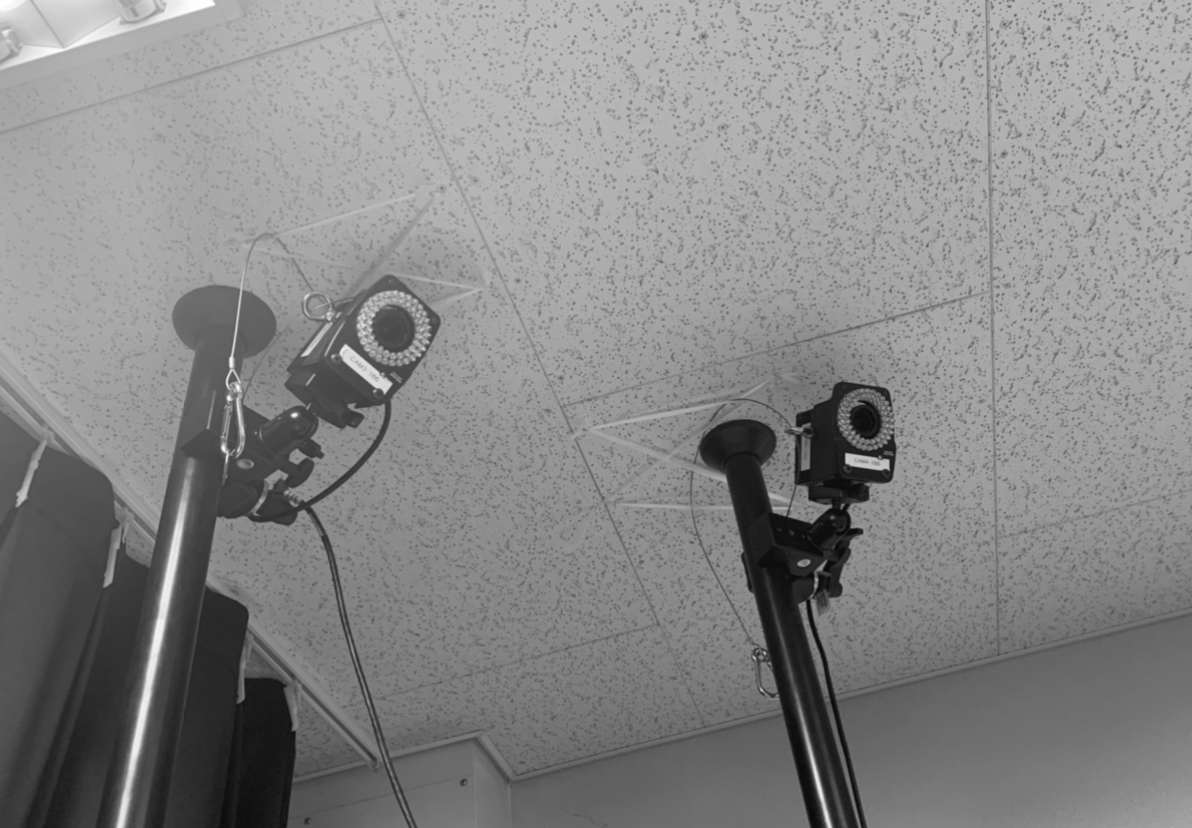
\includegraphics[width=0.9\hsize]{img/camera.jpg}
                \caption{測定に使用するカメラ}
            \end{minipage}
        \end{figure}

        以下に示すようなデータを測定することができる。

        \begin{figure}[h]
            \begin{minipage}{0.5\hsize}
                \centering
                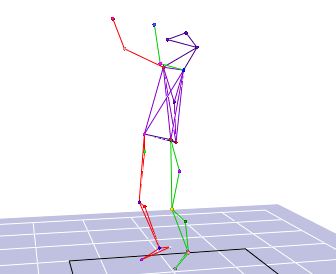
\includegraphics[width=0.9\hsize]{img/form.png}
                \caption{測定されたデータ}
                \label{fig:data}
            \end{minipage}
            \begin{minipage}{0.5\hsize}
                \centering
                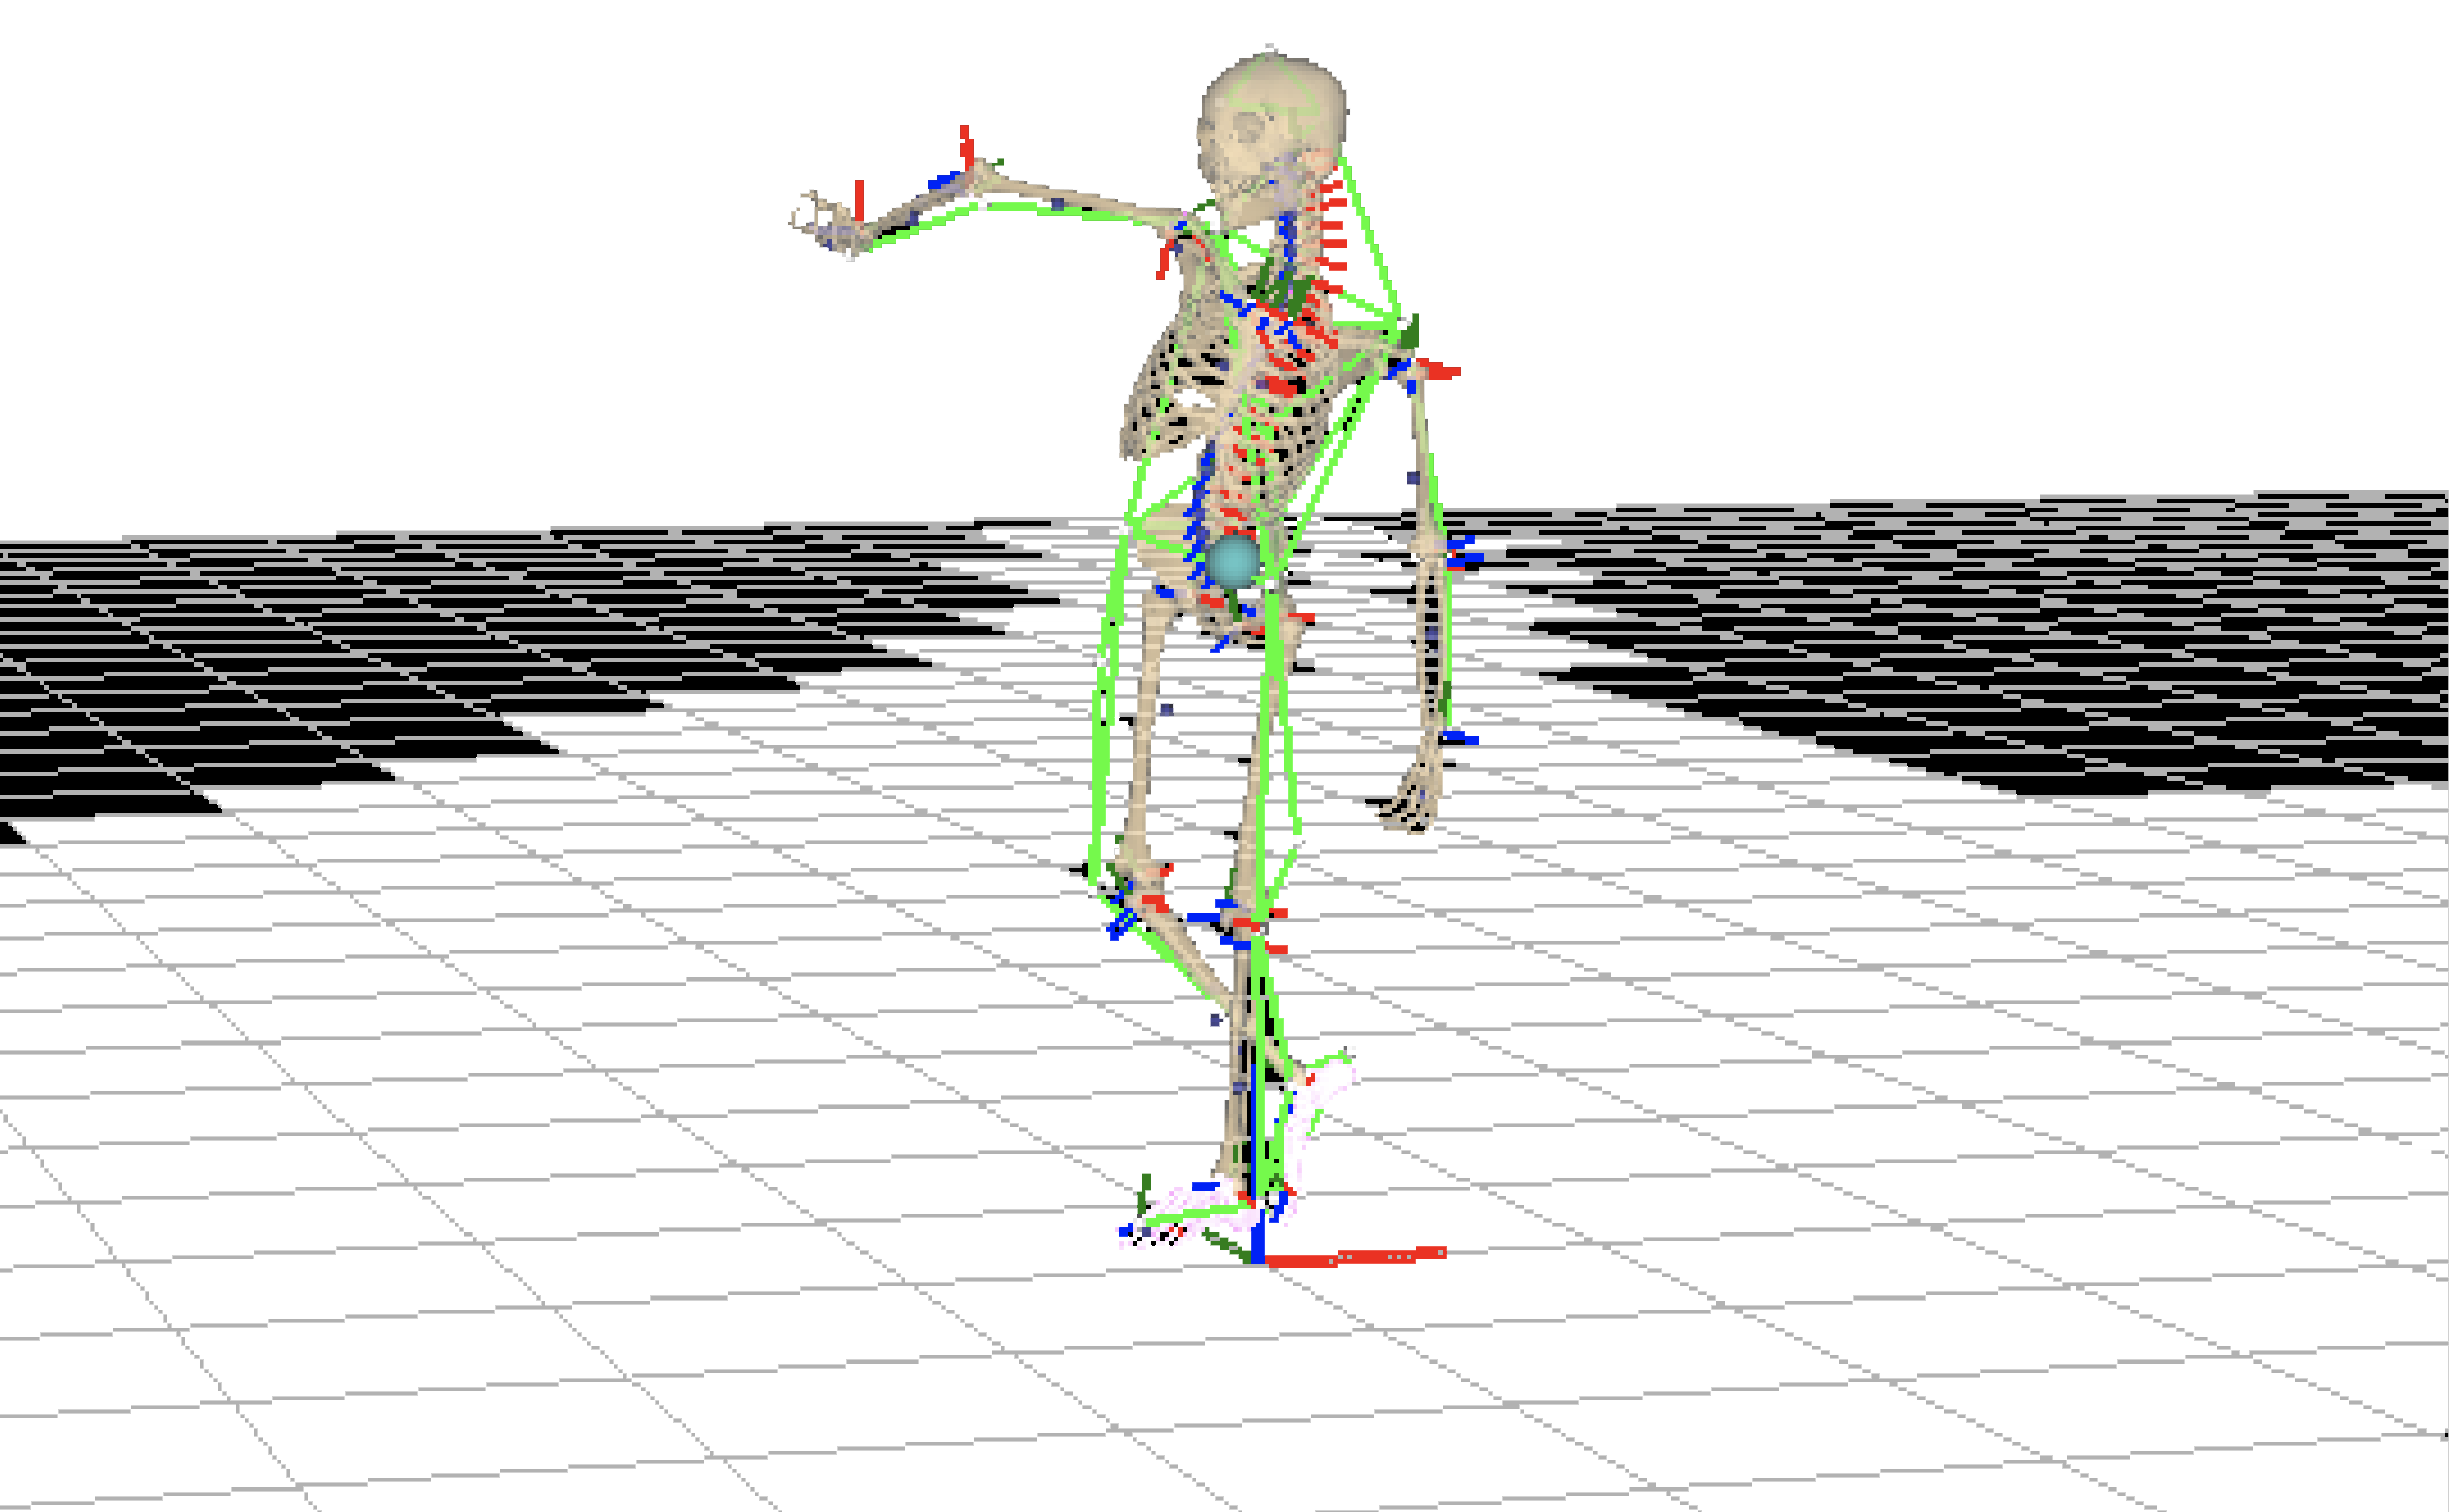
\includegraphics[width=0.9\hsize]{img/spk.png}
                \caption{解析結果}
                \label{fig:anal}
            \end{minipage}
        \end{figure}

        図\ref{fig:data}にあるように、
        実際に被測定者がつけているマーカーがどのように動いていたかを測定することができる。
        さらに、その動きを解析し、図\ref{fig:anal}にあるように各関節に加わる力などが
        子細に見れる。

        \subsection*{長・短所}
            MAC3Dシステムの長所と短所をそれぞれまとめる。

            \paragraph{長所}
                \begin{description}
                    \item[精度] 筋肉、骨の動きなど詳細な解析ができる。
                \end{description}

            \paragraph{短所}
                \begin{description}
                    \item[時間] 計測、解析ともに時間がかかる。リアルタイムでの実用は厳しい。
                    \item[価格] 専用のカメラなど、機材が高価。
                \end{description}

    \section{OpenPose}
        OpenPoseとは、人間の動きの画像から関節の動きを機械学習により推定するシステムである。

        実際に人間の動きに合わせて関節位置を推定している様子を下に示す。
        これは一方向から撮影された画像を解析しているが、
        同時に複数の方向から撮影・分析したデータを用いることで3D化できると考える。

        \begin{figure}[h]
            \centering
            \includegraphics[width=0.6\hsize]{img/op.png}
            \caption{OpenPoseによる関節推定}
        \end{figure}

        \subsection*{長・短所}
            OpenPoseの長所と短所をそれぞれまとめる。

            \paragraph{長所}
                \begin{description}
                    \item[時間] 撮影に準備が不要。高性能なPCがあればリアルタイムな解析も可能。
                    \item[手軽] 専用の機材は要らず、一般的なカメラで撮影可能。
                \end{description}

            \paragraph{短所}
                \begin{description}
                    \item[精度] マーカーなどを使用しないため、挙動が不安定な場合がある。
                \end{description}
        
\end{document}